
\begin{figure}
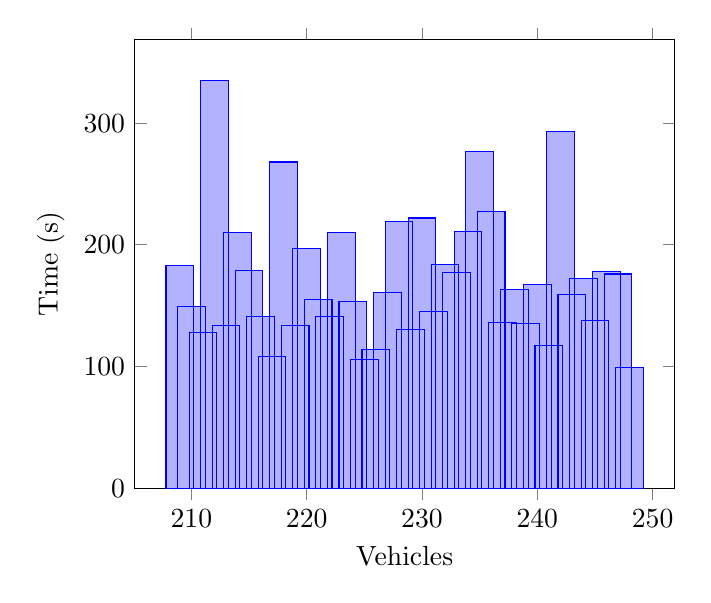
\begin{tikzpicture}
\begin{axis}[
legend style={anchor=west},
xlabel=Vehicles,
ylabel=Time (s),
ymin=0,
ybar,
]
\addplot coordinates {
(248, 99)
(238, 163)
(239, 135)
(234, 211)
(235, 277)
(236, 227)
(237, 136)
(231, 145)
(232, 184)
(233, 177)
(230, 222)
(228, 219)
(245, 138)
(244, 172)
(247, 176)
(246, 178)
(241, 117)
(240, 167)
(243, 159)
(242, 293)
(221, 155)
(215, 179)
(222, 141)
(218, 268)
(219, 134)
(209, 183)
(216, 141)
(217, 108)
(214, 210)
(212, 335)
(213, 134)
(210, 149)
(211, 128)
(229, 130)
(227, 161)
(226, 114)
(225, 106)
(224, 153)
(223, 210)
(220, 197)
};

\end{axis}
\end{tikzpicture}
\label{tik:time:100:97}
\caption{100 percent diving with GSC on route $97$}
\end{figure}
